\documentclass[11pt,a4paper,titlepage]{article}
\usepackage[utf8]{inputenc}
\usepackage[spanish]{babel}
\usepackage{amsmath}
\usepackage{amsfonts}
\usepackage{amssymb}
\usepackage{makeidx}
\usepackage{graphicx}
\usepackage{tipa}
\usepackage{ulem}
\usepackage{multicol}


\title{Report - dUta Proxy Server}
\author{Civile, Juan\ \  \and Sneidermanis, Dario \and Kenny, Kevin}
\date{6 de Junio del 2012}

\begin{document}

\newcommand{\awesome}[1]{\texttt{\large #1}}
\newcommand{\ua}{\textit{User Agent} }
\newcommand{\os}{\textit{Origin Server} }
\newcommand{\duta}{\awesome{dUta} }

\maketitle
\tableofcontents
\clearpage

\section{RFCs consultados}
% {{{

\begin{itemize}

    \item \awesome{RFC 822}  - Standard for the format of ARPA Internet text messages
    \item \awesome{RFC 2119} - Key words for use in RFCs to Indicate Requirement Levels
    \item \awesome{RFC 2396} - Uniform Resource Identifiers (URI): Generic Syntax
    \item \awesome{RFC 1945} - Hypertext Transfer Protocol -- HTTP/1.0
    \item \awesome{RFC 2068} - Hypertext Transfer Protocol -- HTTP/1.1
    \item \awesome{RFC 2616} - Hypertext Transfer Protocol -- HTTP/1.1
    \item \awesome{RFC 2046} - Multipurpose Internet Mail Extensions (MIME) Part Two: Media Types
    \item \awesome{RFC 2047} - MIME (Multipurpose Internet Mail Extensions) Part Three: Message Header Extensions for Non-ASCII Text
    \item \sout{\awesome{RFC 2324} - Hyper Text Coffee Pot Control Protocol (HTCPCP/1.0)}
    \item \awesome{RFC 4627} - The application/json Media Type for JavaScript Object Notation (JSON)
    \item \awesome{RFC 2617} - HTTP Authentication: Basic and Digest Access Authentication
\end{itemize}

% }}}

\section{Protocolo de administración}
% {{{

Para esta seccion, tomamos la sintaxis definida por el RFC 2616 en las secciones 2.1 ``Augmented BNF'' y 2.2 ``Basic Rules''.
También tomamos las definiciones de las secciones 2.5 ``Numbers'' y 2.6 ``Strings'' del RFC 4627.
En caso de definiciones conflictivas, se toma con mayor precedencia las definiciones del RFC 4627.

El protocolo de configuración y monitoreo de \duta utiliza HTTP 1.1 como transporte.
El proxy presenta un servidor HTTP en un puerto especial, este valor es configurable y por defecto es 1337.
Este servidor esta implementando como un filtro mas del proxy, y por lo tanto, soporta todas las mismas funcionalidades HTTP que el proxy.

Los mensajes que recibe y envía este servidor son del tipo \textit{application/json}, como definido en el RFC 4627.
También se hara uso de la \textit{Basic Authentication Scheme} definida en el RFC 2617.
Cualquier recurso o mensaje que no esté detallado en la siguiente sección, producirá un status code de error correspondiente.

\subsection{Nuevo filtro}
\label{sec:new-filter}
Para configurar nuevos filtros se debe hacer un request \awesome{POST} al recurso \awesome{/filter} con un mensaje del formato \textit{filter}.
De ser agregado correctamente, la respuesta tendrá status code 201 y especificará mediante \textit{Location} el recurso asociado al nuevo filtro.
En caso de encontrar un error con el mensaje enviado, se retornara un status code 400, y de ser posible, un mensaje que indique el error.

\begin{verbatim}
filter =
    ("{ 'type': " type ", 'apply': " apply "}") |
    ("{ 'type': " type ", 'apply': " apply ", 'config': " config "}")

type =
    "'deny-all'" |
    "'deny-ip'" |
    "'deny-url'" |
    "'deny-type'" |
    "'deny-size'" |
    "'l33t'" |
    "'rotate'"

apply = "[" apply-rules "]"

apply-rules =
    apply-rule |
    (apply-rule ", " apply-rules)

apply-rule =
    "{ 'ip': " string "}" |
    "{ 'browser': " browser "}" |
    "{ 'os': " os "}"

\end{verbatim}

\textit{browser} es un string con uno de los siguientes valores:

\begin{multicols}{4}

    \small \texttt{APPLE\_MAIL}

    \small \texttt{BOT}

    \small \texttt{CAMINO}

    \small \texttt{CAMINO2}

    \small \texttt{CFNETWORK}

    \small \texttt{CHROME}

    \small \texttt{CHROME\_MOBILE}

    \small \texttt{CHROME10}

    \small \texttt{CHROME11}

    \small \texttt{CHROME12}

    \small \texttt{CHROME13}

    \small \texttt{CHROME14}

    \small \texttt{CHROME15}

    \small \texttt{CHROME16}

    \small \texttt{CHROME17}

    \small \texttt{CHROME18}

    \small \texttt{CHROME19}

    \small \texttt{CHROME8}

    \small \texttt{CHROME9}

    \small \texttt{DOLFIN2}

    \small \texttt{DOWNLOAD}

    \small \texttt{EUDORA}

    \small \texttt{EVOLUTION}

    \small \texttt{FIREFOX}

    \small \texttt{FIREFOX1\_5}

    \small \texttt{FIREFOX10}

    \small \texttt{FIREFOX11}

    \small \texttt{FIREFOX12}

    \small \texttt{FIREFOX13}

    \small \texttt{FIREFOX2}

    \small \texttt{FIREFOX3}

    \small \texttt{FIREFOX3MOBILE}

    \small \texttt{FIREFOX4}

    \small \texttt{FIREFOX5}

    \small \texttt{FIREFOX6}

    \small \texttt{FIREFOX7}

    \small \texttt{FIREFOX8}

    \small \texttt{FIREFOX9}

    \small \texttt{FLOCK}

    \small \texttt{IE}

    \small \texttt{IE10}

    \small \texttt{IE5}

    \small \texttt{IE5\_5}

    \small \texttt{IE6}

    \small \texttt{IE7}

    \small \texttt{IE8}

    \small \texttt{IE9}

    \small \texttt{IEMOBILE6}

    \small \texttt{IEMOBILE7}

    \small \texttt{IEMOBILE9}

    \small \texttt{KONQUEROR}

    \small \texttt{LOTUS\_NOTES}

    \small \texttt{LYNX}

    \small \texttt{MOBILE\_SAFARI}

    \small \texttt{MOZILLA}

    \small \texttt{NETFRONT}

    \small \texttt{OMNIWEB}

    \small \texttt{OPERA}

    \small \texttt{OPERA\_MINI}

    \small \texttt{OPERA10}

    \small \texttt{OPERA9}

    \small \texttt{OUTLOOK}

    \small \texttt{OUTLOOK\_EXPRESS7}

    \small \texttt{OUTLOOK2007}

    \small \texttt{OUTLOOK2010}

    \small \texttt{POCOMAIL}

    \small \texttt{SAFARI}

    \small \texttt{SAFARI4}

    \small \texttt{SAFARI5}

    \small \texttt{SEAMONKEY}

    \small \texttt{SILK}

    \small \texttt{THEBAT}

    \small \texttt{THUNDERBIRD}

    \small \texttt{THUNDERBIRD10}

    \small \texttt{THUNDERBIRD11}

    \small \texttt{THUNDERBIRD12}

    \small \texttt{THUNDERBIRD2}

    \small \texttt{THUNDERBIRD3}

    \small \texttt{THUNDERBIRD6}

    \small \texttt{THUNDERBIRD7}

    \small \texttt{THUNDERBIRD8}

    \small \texttt{UNKNOWN}

\end{multicols}

\textit{os} es un string con uno de los siguientes valores:

\begin{multicols}{4}

    \small \texttt{ANDROID}

    \small \texttt{ANDROID1}

    \small \texttt{ANDROID2}

    \small \texttt{ANDROID2\_TABLET}

    \small \texttt{ANDROID3\_TABLET}

    \small \texttt{ANDROID4}

    \small \texttt{ANDROID4\_TABLET}

    \small \texttt{BADA}

    \small \texttt{BLACKBERRY}

    \small \texttt{BLACKBERRY\_TABLET}

    \small \texttt{BLACKBERRY6}

    \small \texttt{BLACKBERRY7}

    \small \texttt{GOOGLE\_TV}

    \small \texttt{IOS}

    \small \texttt{iOS4\_IPHONE}

    \small \texttt{iOS5\_IPHONE}

    \small \texttt{KINDLE}

    \small \texttt{KINDLE2}

    \small \texttt{KINDLE3}

    \small \texttt{LINUX}

    \small \texttt{MAC\_OS}

    \small \texttt{MAC\_OS\_X}

    \small \texttt{MAC\_OS\_X\_IPAD}

    \small \texttt{MAC\_OS\_X\_IPHONE}

    \small \texttt{MAC\_OS\_X\_IPOD}

    \small \texttt{MAEMO}

    \small \texttt{PALM}

    \small \texttt{PSP}

    \small \texttt{ROKU}

    \small \texttt{SERIES40}

    \small \texttt{SONY\_ERICSSON}

    \small \texttt{SUN\_OS}

    \small \texttt{SYMBIAN}

    \small \texttt{SYMBIAN6}

    \small \texttt{SYMBIAN7}

    \small \texttt{SYMBIAN8}

    \small \texttt{SYMBIAN9}

    \small \texttt{UNKNOWN}

    \small \texttt{WEBOS}

    \small \texttt{WII}

    \small \texttt{WINDOWS}

    \small \texttt{WINDOWS\_2000}

    \small \texttt{WINDOWS\_7}

    \small \texttt{WINDOWS\_98}

    \small \texttt{WINDOWS\_MOBILE}

    \small \texttt{WINDOWS\_MOBILE7}

    \small \texttt{WINDOWS\_VISTA}

    \small \texttt{WINDOWS\_XP}

\end{multicols}


La definición de \textit{host-string} es mixta.
Debe respetar las reglas de \textit{string} definidas en el RFC 4627 y contener un valor válido según el \textit{host} aceptado por el RFC 2616.

El contenido aceptado por \textit{config} y si debe ser omitido o no, sera determinado por el valor de \textit{type}.
Los valores \textit{deny-all}, \textit{l33t} y \textit{rotate} no deben incluir \textit{config}.
\subsubsection{deny-ip}
\begin{verbatim}
config = host-string
\end{verbatim}

\subsubsection{deny-url}
\begin{verbatim}
config = uri
uri = string
\end{verbatim}

\subsubsection{deny-type}
\begin{verbatim}
config = mime
mime = string
\end{verbatim}

\subsubsection{deny-size}
\begin{verbatim}
config = size
size = int
\end{verbatim}

\subsection{Remover filtros}
Para remover un filtro configurado, se debe enviar un request con método \textit{DELETE} y mensaje vacío al recurso asociado al filtro.

\subsection{Monitoreo}
Para obtener los valores de monitoreo, existirá un recurso por cada posible categoría.
Al enviar un request con método \awesome{GET}, el servidor responderá con el valor correspondiente.
Los mensajes contenidos en las respuestas, todos tendrán el mismo formato, \textit{value}.
\begin{verbatim}
value = "{ 'value': " int "} "
\end{verbatim}

Los recursos disponibles son:
\begin{itemize}
    \item \textit{/stats/bytes}
    \item \textit{/stats/bytes/clients}
    \item \textit{/stats/bytes/servers}
    \item \textit{/stats/filter/type} --- Donde \textit{type} es es el definido en \ref{sec:new-filter}.
    \item \textit{/stats/channels}
    \item \textit{/stats/channels/clients}
    \item \textit{/stats/channels/servers}
\end{itemize}
% }}}

\section{Problemas encontrados}
% {{{
    \subsection{Concurrencia}
    Dada la naturaleza de \duta, opera con un alto nivel de concurrencia bajo stress.
    Esto significa que hay que tener una estrategia comprensiva de locking que evite producir dead locks.

    Inicialmente, nos preocupo el impacto que esto podria tener en la perfomance.
    Entonces, optamos por hacer locking lo mas fino posible, para evitar el overhead de sincronizar donde no era necesario.
    Claramente, esto resulto ser un desafio muy complejo, y trajo muchos problemas dificiles de reproducir y aislar.

    Finalmente, optamos por remover estos locks finos.
    Esto resulto en codigo mas facil de seguir, y un proxy estable sin un verdadero impacto en la perfomance.
    La estrategia final es simple: para todo el scope de un request y su asociado response, existe un lock que todos los componentes asociados utilizan para toda operacion.
    Esto se garantiza a nivel reactor, ya que los handlers exponen dicho lock para que este asegure que su ejecucion ocurra de manera sincronizada.

    \subsection{Manejo de mensajes grandes}
    % And so, file storage came to be

    Como no hay control sobre el tamaño de un mensaje, es posible que llegue un mensaje muy grande al servidor.
    Si simplemente lo tuvieramos en memoria, podria tener un serio impacto en el proxy.

    Para solucionar esto, creamos una abstraccion llamada \texttt{DataBuffer}.
    Esta permite utilizar un buffer de manera transparente, sin saber si esta persistido en memoria o en disco.

    \subsection{Delimitacion de mensajes}
    % On the 3rd day came DataBuffer

    Por una decision de diseño, una vez que se lee informacion a un \texttt{DataBuffer}, esta queda asociada con el request al que pertenece el \texttt{DataBuffer}.
    Resulta que si decidiamos implementar \texttt{pipelining} (que era la intencion), tendriamos problemas de perder datos.
    Por eso cambiamos la forma en la que se leia del \texttt{SocketChannel} para que las lecturas se hagan cuando el dueño del \texttt{DataBuffer} pida los datos.
    En contraste con leer inmediamente que llega el evento read.

    Una vez implementado esto descubrimos que tiene un alto impacto en la perfomance.
    Dado que no se sabe donde termina un \texttt{header} mientras se lo lee, hay que leer de a bytes hasta encontrar el final.
    Es decir: hacer una system call \texttt{read} de a un byte.
    Intentamos solucionar este problema con una abstraccion que oculte el \texttt{SocketChannel}.
    Este haria \textit{buffering}, mitigando el efecto de las lecturas pequeñas.
    Lamentablemente, no llegamos a crear una version lo suficientemente estable como para entrar en la version final.

% }}}

\section{Limitaciones}
% {{{

    \subsection{Transformaciones de mensajes grandes}
    Las transformaciones se aplican obligatoriamente en memoria.
    Esto trae un serio problema cuando el mensaje es muy grande, ya que por mas de que se almacena en disco, para procesarlo hay que cargarlo todo.
    Dependiendo del tamaño del mensaje, puede ocurrir que el proxy se quede sin memoria y por lo tanto, deje de servir pedidos.
    Para mitigar este problema, ofrecemos un parametro por linea de comandos para poner un tamaño maximo a los mensajes cuando aplican transformaciones.

    \subsection{HTTP 1.0}
    Si bien \duta es capaz de entender pedidos y respuestas \texttt{HTTP 1.0}, no es capaz de enviar pedidos a un servidor 1.0.
    Es decir, si un servidor de origen no comprende \texttt{HTTP 1.0}, no vamos a poder servir requests a este con exito.

    \subsection{Multipart MIME types}
    Durante el analisis hecho para el pre-informe, notamos que podriamos procesar tipos \texttt{multipart} y detectar que otros tipos contiene.
    La aplicacion de esto seria que los filtros y transformaciones podria ser aplicados aun cuando no todo el mensaje cumple el requisito necesario.

    \subsection{Retry}
    Con la introduccion de conexiones persistentes, es posible que mientras uno empieza a enviar un pedido por una conexion al mismo tiempo el servidor de origen cierre la misma.
    Dado que esto es normal, y no un error, es corrector reintentar en nombre del cliente que envio el pedido.
    Sin embargo, nosotros no ofrecemos este comportamiento.

    \subsection{Content-Encoding}
    \duta no puede aplicar \texttt{encodings}.
    Normalmente, esto no seria un problema, dado que no es necesario saber que contiene el mensaje para transmitirlo.
    Ahora, si se aplica una transformacion es necesario poder remover el encoding para obtener el mensaje original.

    Para evitar problemas con las transformaciones, cuando llega un pedido al que puede aplicar una, interceptamos el header \texttt{Content-Encoding}.
    Al remover este, nos aseguramos de que el mensaje llegue sin encoding, y podamos procesarlo de ser necesario.

% }}}

\section{Posibles extensiones}
% {{{
    \subsection{Pipelining}
    Una clara mejora de perfomance es la implementacion de \texttt{pipelining}.
    Este permite aprovechar mejor una dada conexion.
    Especialmente si se reusa entre distintos usuarios.

    \subsection{Reducir el footprint de memoria}
    Actualmente, toda la informacion relacionada con un request vive durante todo el transcurso del mismo.
    Sin embargo, mucha de esta informacion deja de ser necesaria en varios puntos.
    Seria bueno poder liberar la memoria que contiene esa informacion una vez que esto pasa.

    \subsection{Worker threads}
    El uso de \texttt{worker threads} nos permitiria escalar mejor frente a transformaciones.
    Al no tenerlos, cada transformacion bloquea un \texttt{reactor} durante todo su transcurso, impactando en la capacidad de \duta de servir otros requests.

    \subsection{Limitaciones}
    La posible extension mas importante de todas, es remover las actuales limitaciones relacionadas con features HTTP.
    Varias de estas impactan en el uso que se le puede dar a \duta como proxy.


% }}}

\section{Conclusiones}
% {{{
    El desarrollo fue desafiante y muy interesante.
    El diseño de un servidor que haga uso de NIO no es asunto trivial, y vimos varias iteraciones del diseño.

    Nos hubiera gustado poder implementar algunas cosas como \texttt{pipelining} y \texttt{buffering}.
    Lamentablemente, estos presentan una dificultad muy alta, y nos encontramos limitados en tiempo.
    Dentro de las limitaciones detalladas en las secciones anterios, creemos que presentamos un proxy estable, funcional, y eficiente.

% }}}

\section{Casos de prueba}
% {{{

    Los scripts mencionados en esta seccion se encuentran bajo \texttt{src/test/scripts}.

    \subsection{\awesome{Firefox 12}}
    Utilizamos una instalacion de \awesome{Firefox 12} con el plugin \awesome{HttpFox}.
    \awesome{HttpFox} nos permite revisar los pedidos enviados por \awesome{Firefox} y las respuestas dadas por \duta.

    Una vez configurado \awesome{Firefox} para utilizar el proxy, procedimos a cargar:
    \begin{itemize}
        \item http://www.google.com.ar/
        \item http://www.terra.es/
        \item http://www.facebook.com/
        \item http://en.wikipedia.org/wiki/Casa
        \item http://www.clarin.com.ar/
        \item http://www.ole.com/
        \item http://www.lanacion.com.ar/
    \end{itemize}

    Usando \awesome{HttpFox} podemos verificar que todos los requests tengan respuestas.

    \subsection{Bloqueo por URI}
    Bloqueamos para la IP 127.0.0.1 el acceso a las URIs que contienen \textit{google}.
    Luego probamos ingresar a varios sitios con ese texto, y otros que no.
    Los resultados esperados son:

    \begin{itemize}
        \item http://www.google.com/
        \item http://www.google.com.ar/
        \item http://www.facebook.com/google
        \item http://www.facebook.com/
    \end{itemize}

    Este test se puede reproducir con el script \texttt{block-google.sh}.

    \subsection{Rotacion de imagenes}
    Transformamos para la IP 127.0.0.1 las imagenes, y las rotamos 180 grados.
    Para verificar el efecto accedemos a \texttt{http://www.wikipedia.org}.

    Este efecto se puede generar ejecutando \texttt{add-filter rotate\ ""\ "ip"\ "127.0.0.1"}, y luego ingresando al sitio en un browser que haga uso del proxy en la ip adecuada.

    \subsection{Bloqueo total por browser}
    Probamos el bloqueo por browser con \texttt{Firefox 12} y \texttt{monits.com (190.2.7.69)}.

    Ejecutamos \texttt{add-filter\ "deny-ip"\ "190.2.7.69"\ "browser"\ "FIREFOX12"} y probamos de ingresar con \texttt{Firefox} a \texttt{monits.com}.
    Esto deberia resultar en un error \texttt{404}.
    Sin embargo, ingresar a cualquier otro sitio, deberia cargar normalmente.

    \subsection{Stress test}
    Usamos \texttt{JMeter} para probar la capacidad bajo carga de \duta.
    Esta prueba requiere el script \texttt{dUta stresser.jmx}, y un servidor \texttt{nginx} o \texttt{apache}, configurados para alta capacidad.

    Previamente a descubrir la inestabilidad del parche de \textit{buffering}, tomamos las siguientes mediciones:


    Luego, obtuvimos los siguientes resultados:



% }}}

\newpage

\section{Diseño}
% {{{

	\begin{figure}[ht]
    		\centering
    		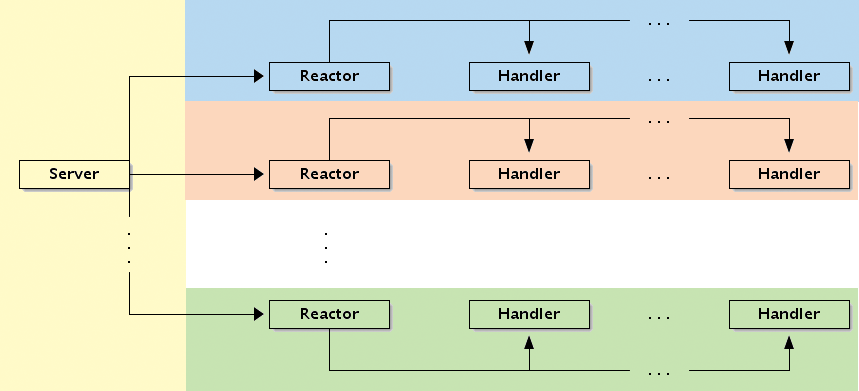
\includegraphics[width=\textwidth]{img/server_reactor_diagram_pro.png}
    		\caption{patrón reactor, en donde hay un Server en su propio thread escuchando todos los
                     sockets y despachando eventos a los Reactors (cada uno en su thread), que se encargan
                     de manejarlos (delegan el trabajo a un Handler).}
	\end{figure}

    \vspace{2cm}

	\begin{figure}[ht]
    		\centering
    		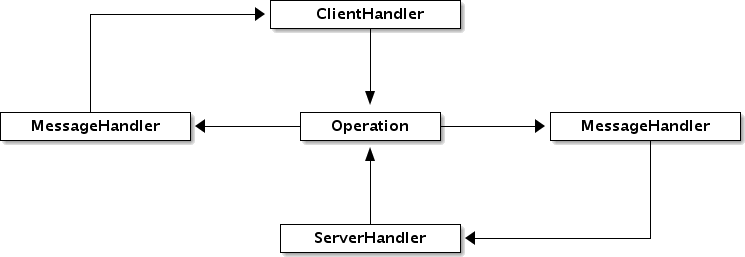
\includegraphics[width=\textwidth]{img/handler_diagram_pro.png}
    		\caption{tanto el ClientHandler como el ServerHandler hacen el procesamiento mínimo para
                     ceder el grueso del trabajo a Operation}
	\end{figure}

	\begin{figure}[ht]
    		\centering
    		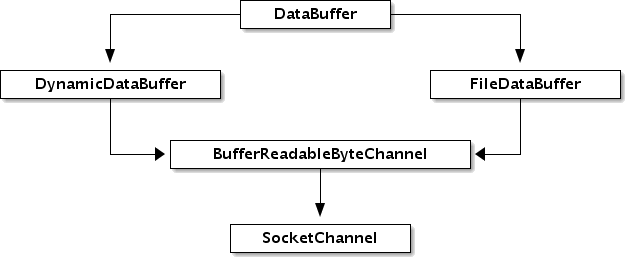
\includegraphics[width=\textwidth]{img/buffer_diagram_pro.png}
    		\caption{el DataBuffer abstrae el uso de un DynamicDataBuffer (datos en RAM) o un
                     FileDataBuffer (datos en disco), que leen datos de entrada de un
                     BufferedReadableByteChannel (buffereo del input del SocketChannel)}
	\end{figure}
% }}}

\newpage

\section{Deploy}
% {{{
    \subsection{Build}
    Para el proceso de build utilizamos la herramienta \awesome{Maven}.
    Simplemente ejecutar \texttt{mvn clean install} genera un archivo \textit{.jar} listo para ejecutar \duta.
    El archivo se encontrara bajo la carpeta \textit{target} y tendra el nombre \textit{dUta-1.0-SNAPSHOT-jar-with-dependencies.jar}.

    \subsection{Logs}
    \duta por defecto utiliza 2 logs.
    Uno es \textit{access.log} que registra todos los pedidos servidos por el proxy.
    El otro es \textit{debug.log}, que registra las acciones tomadas por el proxy.

    Esta configuracion puede ser cambiada editando \textit{src/main/resources/log4j.properties}.
    Recomendamos desactivar \textit{debug.log} a la hora de hacer benchmarking.
    Si bien no tiene un impacto importante en la perfomance, en el evento de que \textit{log4j} rote \textit{debug.log} se ve una caida temporal en la perfomance.

    \subsection{Ejecutar \duta}
    Una vez que se tiene la configuracion de log deseada, y se genera el binario con \awesome{Maven}, estamos listo para ejecutar \duta.
    Simplemente ejectuar \texttt{java -jar target/dUta-1.0-SNAPSHOT-jar-with-dependencies.jar} inicia el proxy con la configuracion por defecto.

    \subsubsection{Argumentos}
    Opcionalmente, se pueden pasar argumentos por linea de comandos que cambian los valores de configuracion por defecto.
    \begin{verbatim}
        --chain=ip:port    Chain to another proxy
        --port=port        Listen for requests on `port`
        --admin-port=port  Listen for admin requests on `port`
        --size-limit=size  Limit the size of files for transforms
    \end{verbatim}

    A motivo de ejemplo, mostramos como ejecutar \duta para que se conecte a un segundo proxy corriendo en la misma pc.
    Asumamos que el segundo proxy ya esta utilizando el puerto 9999.
    Por lo tanto, hay que proveer a \duta de un puerto libre para escuchar, en este caso usaremos el 8888.

    Para ejecutar con esta configuracion corremos (saltos de linea introducidos por legibilidad):
    \begin{verbatim}
        java
            -jar target/dUta-1.0-SNAPSHOT-jar-with-dependencies.jar
            --port=8888
            --chain=localhost:9999
    \end{verbatim}

    \subsection{Administracion}
    Una vez que el servidor esta corriendo, se puede utilizar el protocolo de configuracion.

    Por ejemplo, para agregar un filtro que bloquee todos los requests hechos desde \textit{localhost}, podemos ejecutar:
    \begin{verbatim}
        curl
            -vvv
            -d '{"type": "deny-all", "apply": [{"ip": "127.0.0.1"}]}'
            -H "Content-Type: application/json"
            --basic --user "heman:masterofuniverse"
            localhost:1337/filters
    \end{verbatim}


% }}}

\end{document}
